%Copyright (c) 2004 2005 2006 Atos Origin
%Permission is granted to copy, distribute and/or modify this
%document
%under the terms of the GNU Free Documentation License,
%      Version 1.2
%      or any later version published by the Free Software
%      Foundation;
%      with no Invariant Sections, no Front-Cover
%      Texts, and no Back-Cover
%      Texts.  A copy of the license is
%      included in the section entitled "GNU
%      Free Documentation License".
%
%$Id: eval.tex,v 1.1 2006/02/16 16:33:33 goneri Exp $
\section{Evaluate}
\begin{figure}
\center
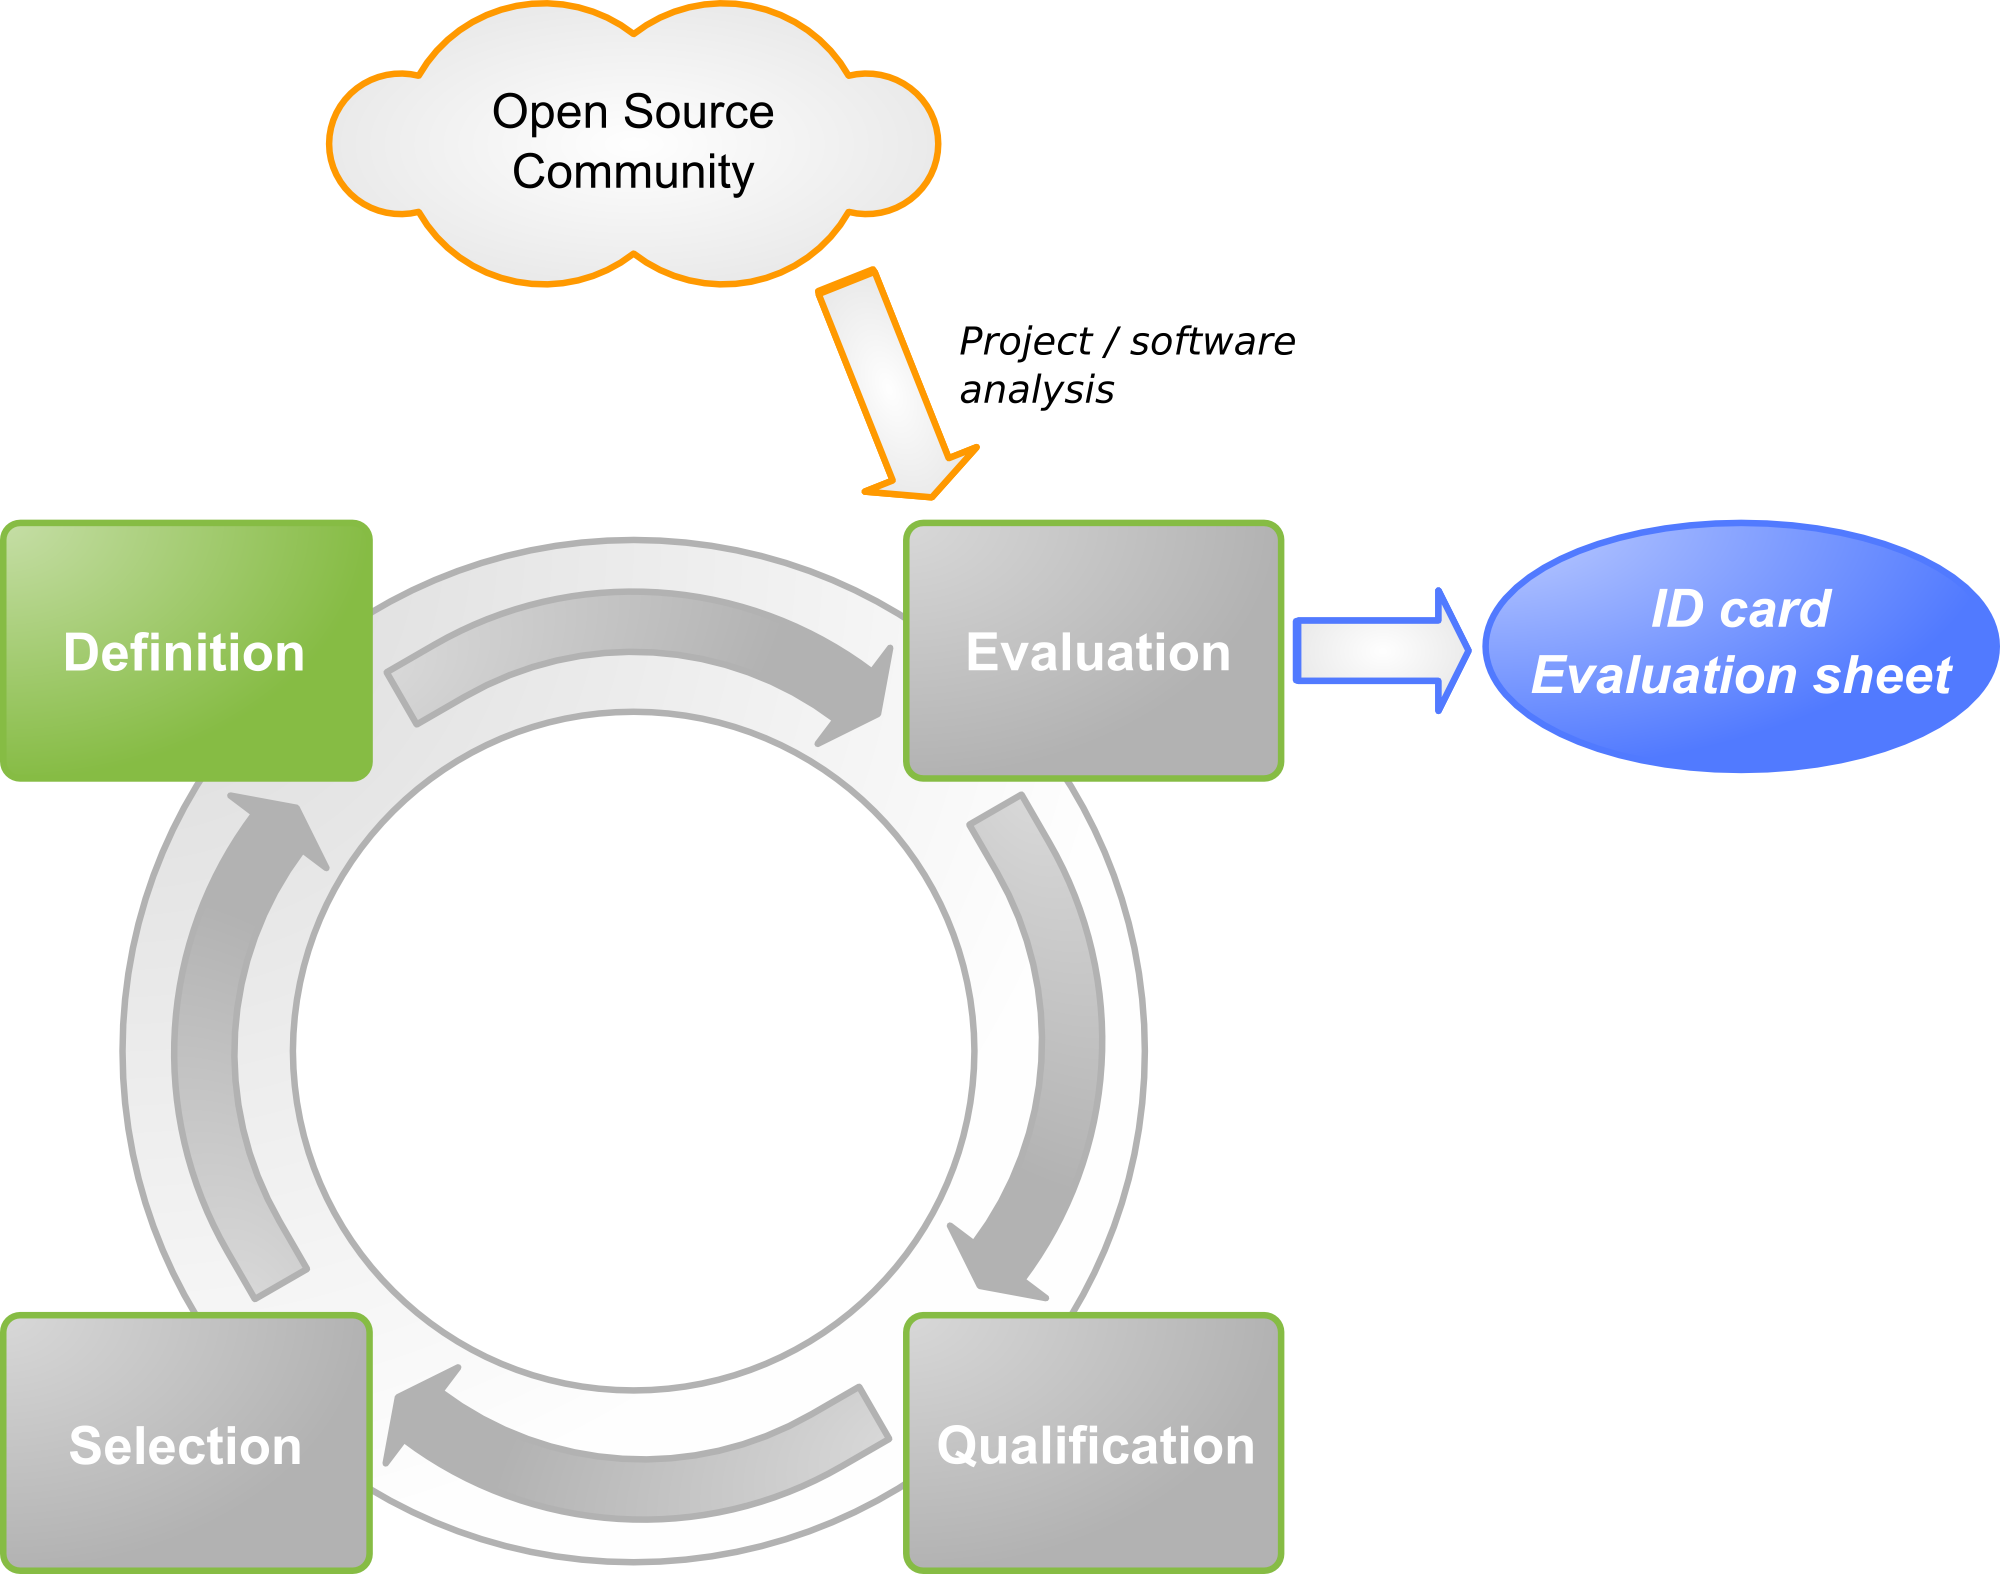
\includegraphics[width=13cm]{images/evaluer}
\caption{Step 2 - Evaluate}
\end{figure}


\subsection{Objective}
The objective of this step is to carry out the evaluation of the software. It consists in collecting information from the open source community, in order to:

\begin{itemize}
\item Build the identity card of a softwarev
\item Build the evaluation sheet of a software, by scoring tcriteria split on three major axis:
  \begin{itemize}
  \item Functional coverage
  \item Risks from user's perspective
  \item Risks from service provider's perspective
  \end{itemize}
\end{itemize}

This evaluation effort can be inserted in a more global approach of technological survey which is not completely described in this document.

\subsection{Identity card}
Data constituting the identity card is raw and factual and is not directly scored. Howerver it is used as a basis for the scoring process described below.


The main parts of an identity card are:


\subsubsection{General information}
\begin{itemize}
\item Name of the software
\item Reference, date of creation, date of release of the ID card
\item Author 
\item Type of software 
\item Brief description of the software
\item Licenses to which the software is subjected
\item Project's URI and demonstration site
\item Compatible operating systems
\item Fork's origin (if the software is a fork)
\end{itemize}

\subsubsection{Existing services}
\begin{itemize}
\item Documentation
\item Number of contractual support offers
\item Number of training offers
\item Number of consultancy offers
\end{itemize}

\subsubsection{Functional and technical aspects}
\begin{itemize}
\item Technologies of implementation
\item Technical prerequisites
\item Detailed functionalities
\item Roadmap
\end{itemize}

\subsubsection{Synthesis}
\begin{itemize}
\item General trend
\item Comments
\end{itemize}
